\subsubsection{Metodología}
Este proyecto se ha llevado a cabo mediante la metodología SCRUM. Por lo que semanalmente se ha procurado tener un producto entregable, iterando en este y mejorándolo. Esto se verá reflejado en el orden de realización de tareas. Para organizar dichas tareas se ha usado Obsidian con el plugin Kanban, así se mantiene el orden de las mismas, qué hay que hacer y qué queda por hacer.

\subsubsection{Librería de InputStick}
Para la comunicación con InputStick es necesario importar la librería de InputStick\cite{sticklibrary} al proyecto. Como está escrita en Java y la aplicación de Bitwarden está escrita en Xamarin (C\#) habrá que usar un intermediaro para realizar la comunicación, para esto usaremos \gls{jbl}\cite{bindingjar} en VisualStudio, que nos permitirá importar el .jar que es la librería de InputStick.\footnote{\href{https://github.com/PabloOQ/mobile/commit/40e370ec8dcce3fb693363a26eb971239fb9728a}{Bindings library 1}, \href{https://github.com/PabloOQ/mobile/commit/d6cccb783599da01ed99baa2ad924bea75dbf7d9}{Bindings library 2}}

\subsubsection{Código}
En esta sección hablaremos del código más relevante, hemos dejado fuera algunas partes de las implementaciones de las interfaces de las que se habla, así como la parte Vista y Vista-Modelo, sólo se discutirá el Modelo, por supuesto el resto del código se encuentra en el repositorio. \ref{repos}

El código se ha escrito desde la base de que InputStick es un proveedor de escritura automática, pero pueden haber varios. Por ello, aunque actualmente sólo haya uno, en los ajustes hay un selector del proveedor, en vez de un botón para alternar activado y desactivado. Al proveedor se le debe proporcionar toda la información necesaria cada vez que se quiere escribir, este no almacena nada, excepto lo necesario para realizar conexiones, que es específico al proveedor. Podemos verlo en su interfaz:
\begin{csharp}[firstnumber=6]{src/Core/Abstractions/IAutoTyperProvider.cs}
namespace Bit.Core.Abstractions
{
    public interface IAutoTyperProvider
    {
        void Connect();
        void Disconnect();
        void Type(string text, LayoutType layout, SpeedType speed);
    }
}
\end{csharp}

Así que hemos creado un servicio AutoTyper, este servicio se ocupa de guardar y cargar datos persistentes, aunque realmente es un intermediario, así puede interceptar la información, y validarla. Esto lo hacemos por si un proveedor ya no es compatible con una disposición o se elimina el soporte para un proveedor. Si esta información es errónea o nunca ha sido configurada por el usuario se le otorga un valor por defecto.

\begin{csharp}[firstnumber=7]{src/Core/Abstractions/IAutoTyperService.cs}
namespace Bit.Core.Abstractions
{
    public interface IAutoTyperService
    {
        IAutoTyperWrapper GetTyperWrapper();

        Task InitAsync();

        Task<AutoTyperProviderType> GetProviderTypeAsync();
        Task SetProviderAsync(AutoTyperProviderType type);
        Task<LayoutType> GetLayoutAsync(AutoTyperProviderType type);
        Task SetLayoutAsync(LayoutType layout, AutoTyperProviderType type);
        Task<SpeedType> GetSpeedAsync(AutoTyperProviderType type);
        Task SetSpeedAsync(SpeedType speed, AutoTyperProviderType type);

        List<AutoTyperProviderType> GetCompatibleProviders();
        List<LayoutType> GetCompatibleLayouts(AutoTyperProviderType type);
        List<SpeedType> GetCompatibleSpeeds(AutoTyperProviderType type);

        IAutoTyperProvider CreateTyper(AutoTyperProviderType? type);
        AutoTyperProviderType ProviderType(IAutoTyperProvider? provider);
    }
}
\end{csharp}

Aquí el proveedor de auto escritura se asegura de devolver datos válidos:
\begin{csharp}[firstnumber=32]{src/Android/Services/AutoTypers/AutoTyperService.cs}
...
    public async Task<AutoTyperProviderType> GetProviderTypeAsync()
    {
        var provider = (AutoTyperProviderType?) await _stateService.GetAutoTyperProviderAsync();
        return provider ?? AutoTyperProviderType.None;
    }
...
\end{csharp}

El servicio de estados es el que realmente se ocupa de guardar los datos, los cuales son locales, pero individuales a cada cuenta en el dispositivo, este al recoger la información se asegura que esté definida, si no lo está devuelve nulo y se le relega solucionar el problema a quien realiza la llamada, que siempre es nuestro servicio intermediaro AutoTyper.
\begin{csharp}[firstnumber=1318]{src/Core/Services/StateService.cs}
...
    public async Task<int?> GetAutoTyperProviderAsync(string userId = null)
    {
        var reconciledOptions = ReconcileOptions(new StorageOptions { UserId = userId },
            await GetDefaultStorageOptionsAsync());
        var key = Constants.AutoTyperProviderKey(reconciledOptions.UserId);
        int? provider = await GetValueAsync<int?>(key, reconciledOptions);
        // Check if provider is valid
        if (provider != null && !Enum.IsDefined(typeof(AutoTyperProviderType), (byte)provider))
        {
            provider = null;
        }
        return provider;
    }
...
\end{csharp}

Adicionalmente al recoger las disposiciones y velocidades siempre se debe devolver un valor concreto, no existe \quotes{Ninguna disposición} ni \quotes{Ninguna velocidad}. Por ello el servicio de auto escritura se solicita a sí mismo las opciones compatibles y contrasta el valor por defecto con esta lista, ya que un proveedor puede no ser compatible con ese valor, si no lo es elegimos un valor cualquiera, en este caso el primer elemento de la lista.

\begin{csharp}[firstnumber=107]{src/Android/Services/AutoTypers/AutoTyperService.cs}
...
        // Helpers

        /**
         * Checks if the element is in the list
         * If not, it defaults to def
         * If def is not in the list, it defaults to the first element of the list  
         */
        private static T Validate<T>(T element, List<T> list, T def)
        {
            return FindOrDefault(FindOrDefault(element, list, def), list, list[0]);
        }

        /**
         * Checks if the element is in the list
         * If not, it defaults to def
         */
        private static T FindOrDefault<T>(T element, List<T> list, T def)
        {
            return list.Contains(element) ? element : def;
        }
    }
}
\end{csharp}


Al servicio de auto escritura se le puede solicitar un contenedor de proveedor, esta es la única forma de contactar con el proveedor, así forzamos a que cuando se vaya a enviar algo para escribir al proveedor los datos ya hayan sido inicializados (proveedor, distribución y velocidad). Y aunque pueden haber varias instancias de la implementación del contenedor, el servicio devolverá siempre la misma instancia cuando se le solicite, de forma similar al patrón singleton, ya que el contenedor actua como una extensión del servicio.
\begin{csharp}[firstnumber=3]{src/Core/Abstractions/IAutoTyperWrapper.cs}
namespace Bit.Core.Abstractions
{
    public interface IAutoTyperWrapper
    {
        Task LoadAsync();
        void Connect();
        void Disconnect();
        void Type(string text);
        bool IsEnabled();
    }
}
\end{csharp}

En nuestro caso hemos usado la librería de InputStick mediante llamadas a la app de InputStickUtility, que se ocupa de mandar los datos a InputStick. Lamentablemente no es lo que se pretendía, pero la falta de tiempo nos ha impedido usar la \gls{api} de InputStick en mayor profundidad. Dicha \gls{api} se puede usar de dos formas:
\begin{itemize}
    \item InputStickBroadcast: Al usar esta parte de la \gls{api} es mucho más simple contactar con InputStick, ya que únicamente es necesario mandar a InputStick qué tiene que escribir, del resto se ocupa InputStickUtility.
    \item Completa: Al usar la \gls{api} en su totalidad se puede evitar la instalación de InputStickUtility, pero es requiere una implementación más compleja ya que las facilidades que otorgaba InputStickUtility ya no están presentes, por ejemplo es necesario saber la dirección \textit{Media Access Control}(MAC)\footnote{Esta es la única vez en este documento que usaremos el acrónimo MAC con un significado distinto a \acrlong{cryptomac}} de InputStick.
\end{itemize}
\begin{csharp}[firstnumber=9]{src/Android/Services/AutoTypers/InputStickBroadcastAndroid.cs}
namespace Bit.Droid.Services.AutoTypers
{
    public class InputStickBroadcastAndroid : IAutoTyperProvider
    {
        public void Connect()
        {
            InputStickBroadcast.RequestConnection(Application.Context);
        }

        public void Disconnect()
        {
            InputStickBroadcast.ReleaseConnection(Application.Context);
        }

        public void Type(String text, LayoutType layout, SpeedType speed)
        {
            InputStickBroadcast.Type(Application.Context,
                text,
                _layouts.ContainsKey(layout) ? _layouts[layout] : _layouts[0], // Should not happen, this is a fallback
                SpeedToValue(speed));
        }
...
\end{csharp}


Para administrar la selección de distribución se usa un enum, este enum contiene todas las disposiciones listadas por InputStick:
\noindent\url{https://github.com/inputstick/InputStickAPI-Android#keyboard-layouts}
\begin{csharp}[firstnumber=3]{src/Core/Enums/LayoutType.cs}
namespace Bit.Core.Enums
{
    public enum LayoutType
    {
        [LocalizableEnum("AutoTyperLayoutCSCZ")]
        cs_CZ = 0,
        [LocalizableEnum("AutoTyperLayoutDADK")]
        da_DK = 1,
...
\end{csharp}

Igualmente para administrar la velocidad de escritura se usa otro enum, este enum es una ampliación de las posibilidades que ofrece InputStick, ya que las apps oficiales de InputStick usan todas las velocidades listadas excepto \quotes{Fast} y \quotes{Faster}. De cara al usuario se usan estos términos y no las velocidades reales dos motivos:
\begin{itemize}
    \item Para no abrumar al usuario: Es innecesario que el usuario sepa las velocidades concretas, mostrar tantos números, en una escala que realmente a las velocidades más altas una persona no es capaz de cuantizar la diferencia, solo lograría sobreestimularlo.
    \item Porque realmente no es consistente: Estas velocidades se han extraído de las apps oficiales de InputStick creando un pequeño script de python en el que medir las velocidades, pues el creador no dice en ningún lugar las velocidades ya que dependen de la carga de trabajo del dispositivo en el que esté conectado. Si el dispositivo está muy sobrecargado la máxima velocidad no funcionará correctamente y el dispositivo no leerá todas las teclas y por tanto se saltará alguna. Por tanto las velocidades descritas son aproximaciones bajo poca carga.
\end{itemize}
\begin{csharp}[firstnumber=3]{src/Core/Enums/SpeedType.cs}
namespace Bit.Core.Enums
{
    public enum SpeedType : int         // keys per second (aproximate) - ratio
    {
        [LocalizableEnum("Slowest")]    // 8 - 0.1
        Slowest = 0,
        [LocalizableEnum("Slower")]     // 16 - 0.2
        Slower = 2,
        [LocalizableEnum("Slow")]       // 40 - 0.5
        Slow = 3,
        [LocalizableEnum("Normal")]     // 80 - 1
        Normal = 5,
        [LocalizableEnum("Fast")]       // 120 - 1.5
        Fast = 7,
        [LocalizableEnum("Faster")]     // 180 - 2.25
        Faster = 6,
        [LocalizableEnum("Fastest")]    // 240 - 3
        Fastest = 10,                   
    }
}
\end{csharp}
\newpage
\subsubsection{Cambios visuales}
En la figura \ref{fig:bitapp-mod} podemos ver los cambios hechos en la GUI. En cada campo que hubiese un botón de copiar al portapapeles se ha añadido el botón de enviar al proveedor de escritura automática, este campo sólo es visible cuando se ha seleccionado un proveedor. También se ha añadido una pantalla de configuración de esta funcionalidad, con selectores de proveedor, idioma y velocidad. Se puede acceder a la pantalla de los ajustes del proveedor de escritura automática desde la pantalla de ajustes.
\begin{figure}[H]
    \centering
    \subfigure[]{\frame{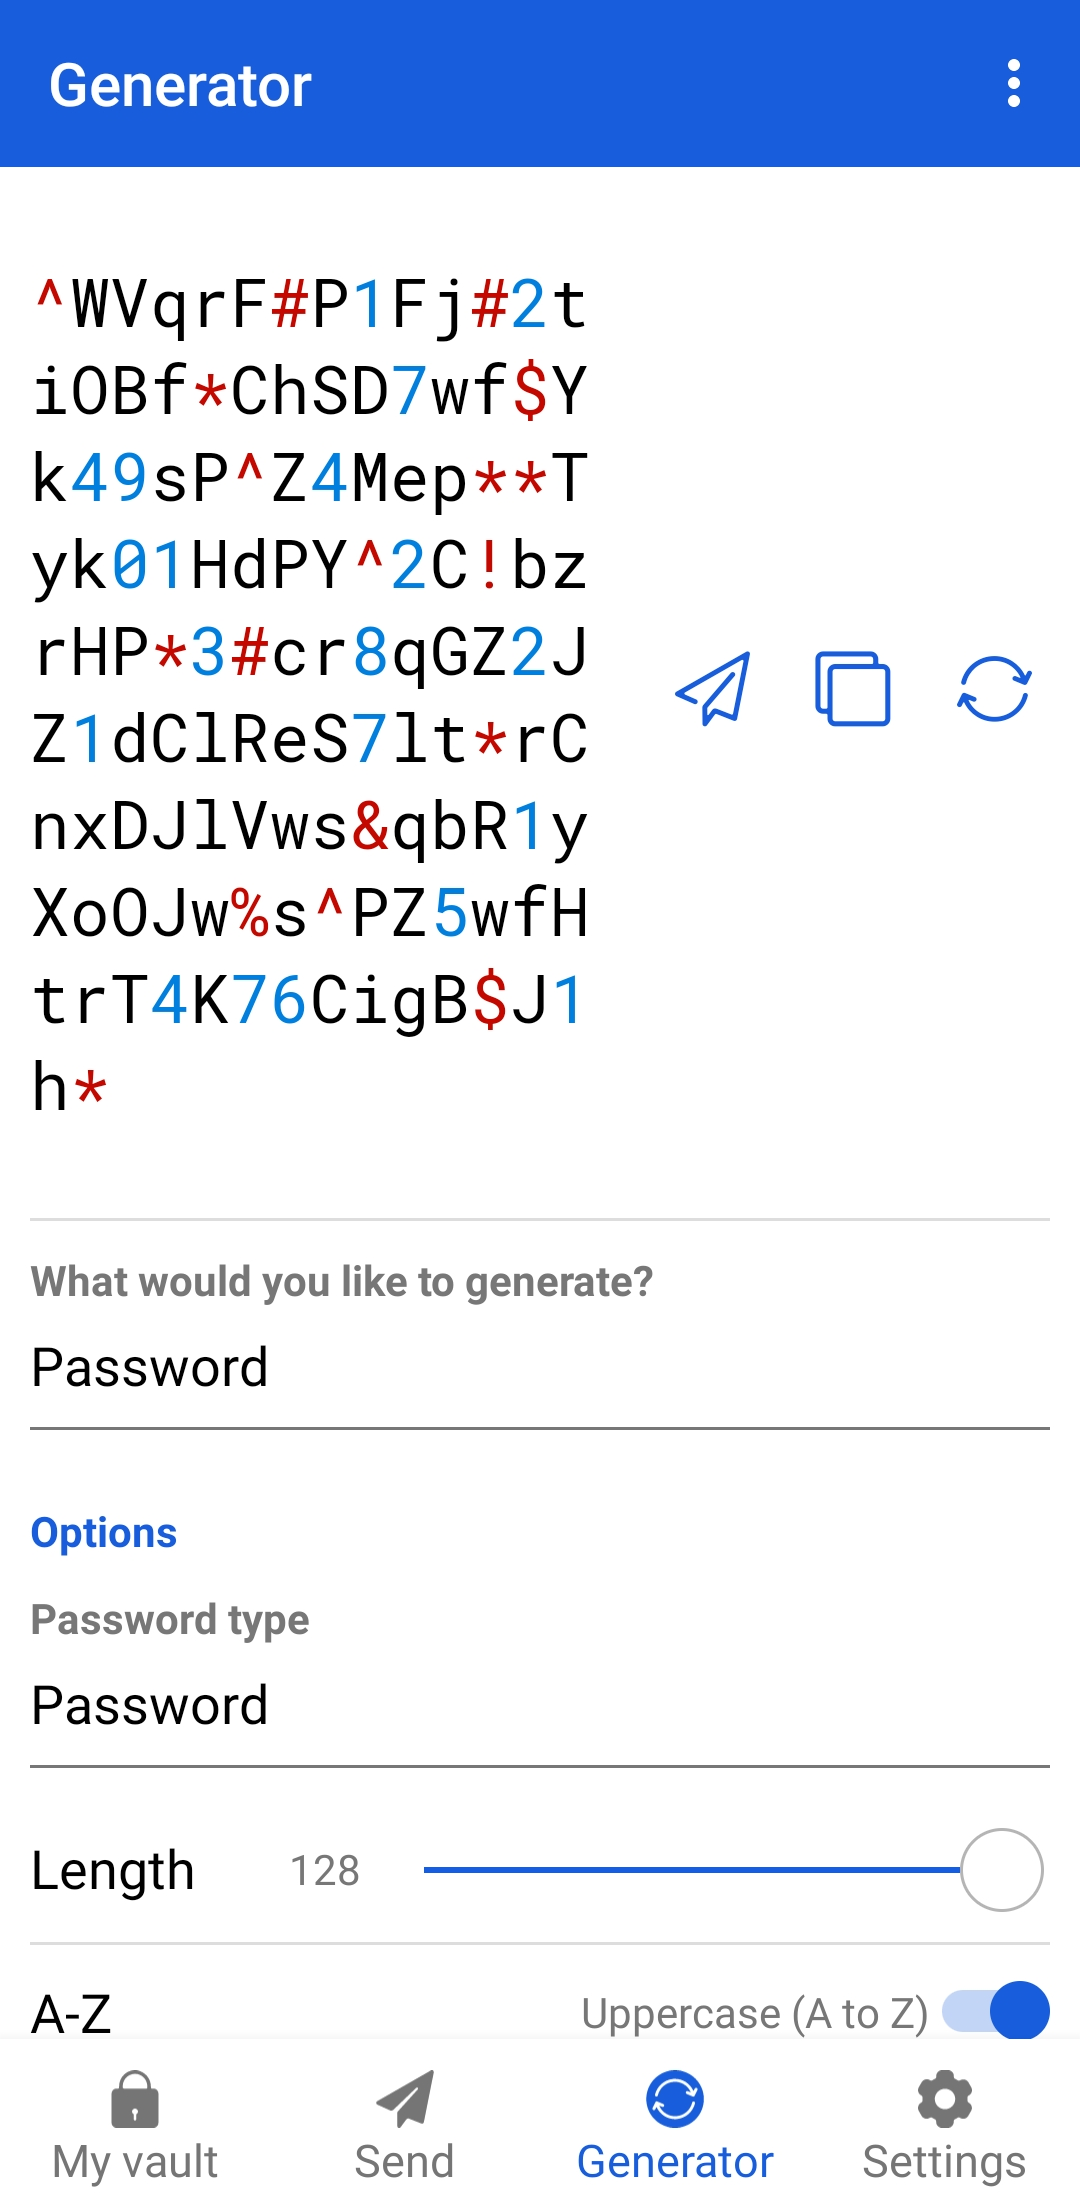
\includegraphics[width=0.4\columnwidth]{gfx/bitapp-mod-generator.png}}}
    \subfigure[]{\frame{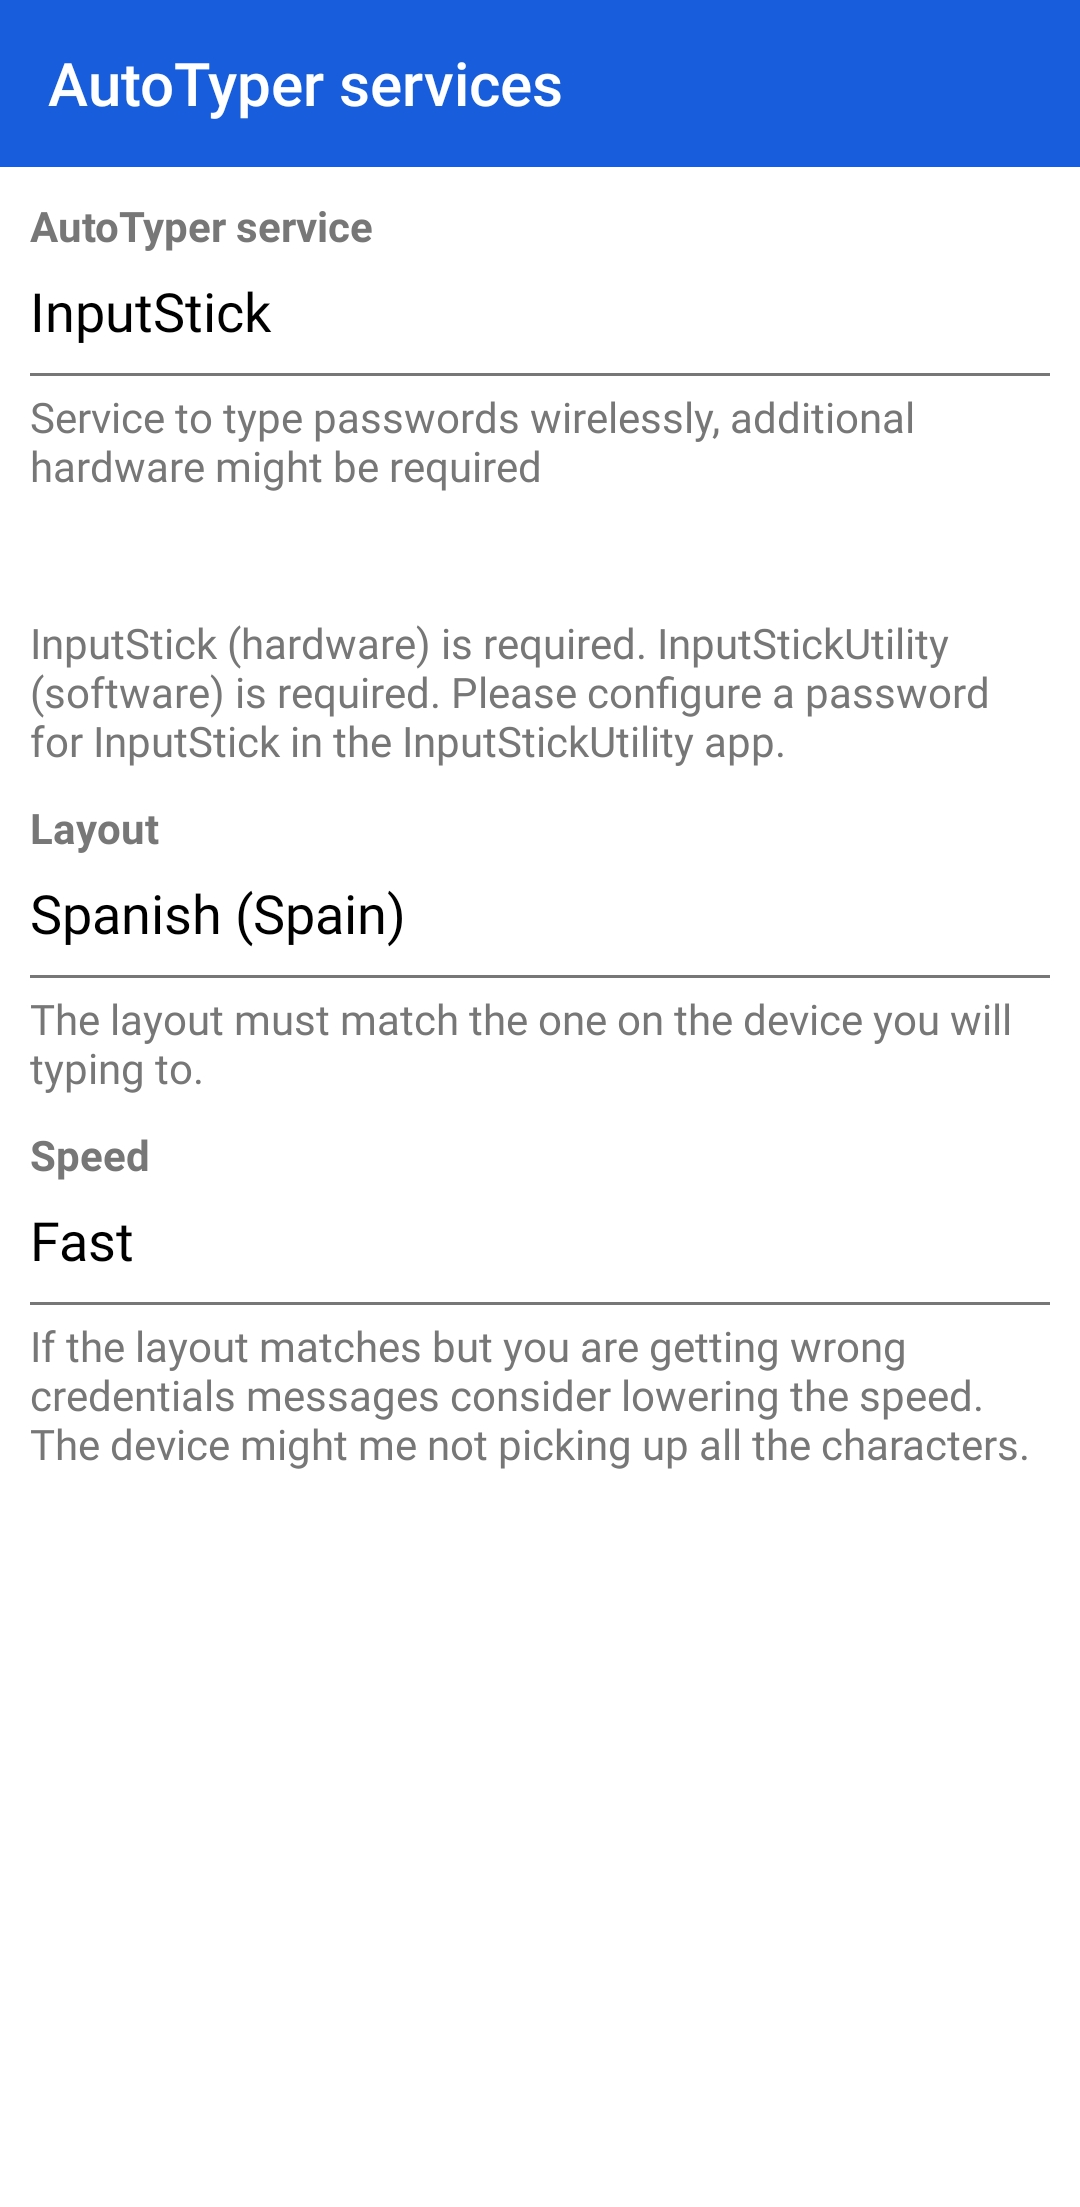
\includegraphics[width=0.4\columnwidth]{gfx/bitapp-mod-settings.png}}}
\caption{
        Figura múltiple. Modificación de la app de Bitwarden. \newline
        \tab (a) Pantalla de generación con el botón de enviar. \newline
        \tab (b) Pantalla de ajustes del proveedor de escritura automática.
        }
    \label{fig:bitapp-mod}
\end{figure}

En la figura \ref{fig:bitapp-mod-login} podemos ver todos los cambios realizados en la pantalla de un \gls{login}. El botón de enviar se encuentra en varios campos, hay que destacar que si un campo se encuentra vacío no hay nada que enviar, por lo que no se mostraría. Tampoco se mostraría si el proveedor de escritura automática se encuentra desactivado.
\begin{figure}[H]
    \centering
    \frame{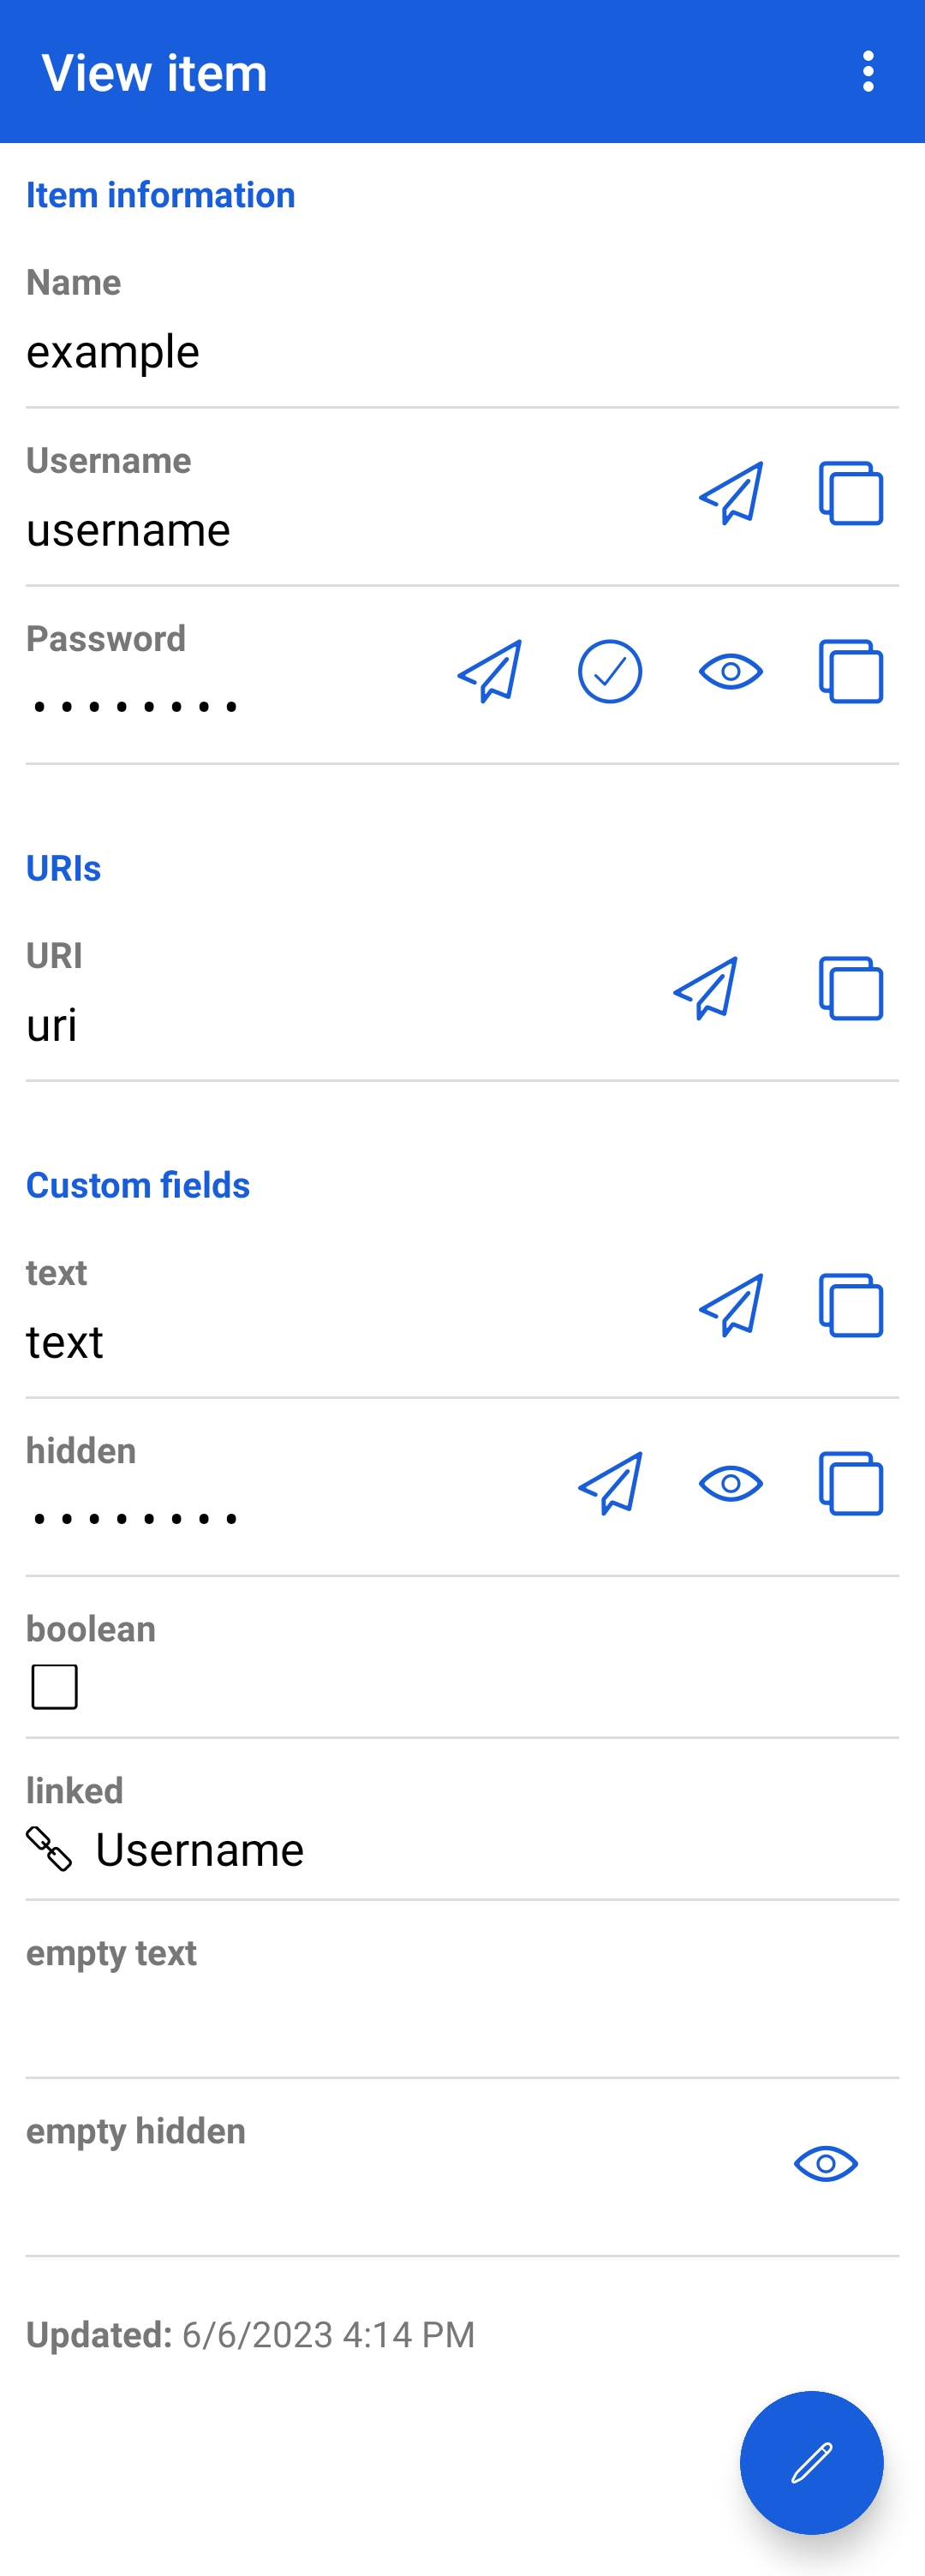
\includegraphics[width=0.4\columnwidth]{gfx/bitapp-mod-login.png}}
\caption{Pantalla de elemento. Modificación de la app de Bitwarden} % no se referencia \gls{login} porque hace que ocupe exactamente una línea más y por lo tanto pasa a la página siguiente
    \label{fig:bitapp-mod-login}
\end{figure}

\subsubsection{Repositorios}\label{repos}
Los cambios realizados se encuentran en el fork de GitHub de PabloOQ.
Debido a un problema de compatibilidad durante el desarrollo hubo que hacer un merge de la rama master de Bitwarden, todo el código se encuentra en:

\noindent\url{https://github.com/PabloOQ/mobile/tree/stick-after-merge}

\noindent Sin embargo, para visualizar rápidamente el código modificado antes de hacer el merge, se podría ver en esta rama (aunque este está también en la rama mencionada anteriormente):

\noindent\url{https://github.com/PabloOQ/mobile/tree/stick}

\noindent Finalmente en este enlace se muestra el código añadido, al ser el total no incluye el código previo a las refactorizaciones.

\noindent\url{https://github.com/PabloOQ/mobile/compare/tfg-diff...PabloOQ:mobile:stick-after-merge}

\noindent El informe escrito en LaTeX se encuentra en:

\noindent\url{https://github.com/PabloOQ/informeTFG}
\newpage

\subsubsection{Plan de trabajo}
En la tabla \ref{tab:plan_original} se muestra el plan de trabajo original.
\begin{table}[H]
\begin{tabular}{|p{0.25\textwidth}|p{0.12\textwidth}|p{0.48\textwidth}|}
\hline
Fases                                & Duración \newline Estimada & Tareas \\ \hline

Estudio previo / Análisis            & 85                & Tarea 1.1: Estudio de la aplicación de Bitwarden \newline Tarea 1.2: Estudio de la \gls{api} de InputStick \\ \hline

Diseño / Desarrollo / Implementación & 85                & Tarea 2.1: Diseño y creación de la interfaz de usuario \newline Tarea 2.2: Adaptar la \gls{api} de InputStick a C\# \newline Tarea 2.3: Implementación de InputStick a Bitwarden \\ \hline

Evaluación / Validación / Prueba     & 30                & Tarea 3.1: Verificación de la \gls{gui} \newline Tarea 3.2: Verificación de la funcionalidad nueva \\ \hline

Documentación / Presentación         & 100               & Tarea 4.1: Documentación de la \gls{gui} \newline Tarea 4.2: Documentación de la funcionalidad nueva \newline Tarea 4.3: Documentación de temas relacionados \\ \hline
\end{tabular}
\caption{Plan de trabajo original. Realización propia.}
\label{tab:plan_original}
\end{table}

Sin embargo realmente las horas dedicadas son las que se muestran en la tabla \ref{tab:plan_real}. Esto cambio se debe a que el estudio de la aplicación fue mucho más complejo de lo esperado y por tanto requirió mucho más tiempo.

\begin{table}[H]
\begin{tabular}{|p{0.25\textwidth}|p{0.12\textwidth}|p{0.48\textwidth}|}
\hline
Fases                                & Duración \newline Estimada & Tareas \\ \hline

Estudio previo / Análisis            & 115               & Tarea 1.1: Estudio de la aplicación de Bitwarden \newline Tarea 1.2: Estudio de la \gls{api} de InputStick \\ \hline

Diseño / Desarrollo / Implementación & 85               & Tarea 2.1: Diseño y creación de la interfaz de usuario \newline Tarea 2.2: Adaptar la \gls{api} de InputStick a C\# \newline Tarea 2.3: Implementación de InputStick a Bitwarden \\ \hline

Evaluación / Validación / Prueba     & 15                & Tarea 3.1: Verificación de la \gls{gui} \newline Tarea 3.2: Verificación de la funcionalidad nueva \\ \hline

Documentación / Presentación         & 85               & Tarea 4.1: Documentación de la \gls{gui} \newline Tarea 4.2: Documentación de la funcionalidad nueva \newline Tarea 4.3: Documentación de temas relacionados \\ \hline
\end{tabular}
\caption{Plan de trabajo real. Realización propia.}
\label{tab:plan_real}
\end{table}